\chapter{Background and Literature Review}

In the fashion industry, \acs{AI} is applied to a range of tasks and objectives, including analysis, recommendation and synthesis, among others as described in \cite[cf.]{chen_survey_2023}, \cite[cf.]{deldjoo_review_2022}, \cite[cf.]{kouslis_ai_2024} and \cite[cf.]{cheng_fashion_2020} and as illustrated in Figure \ref{fig:fashion-areas}.

\begin{figure}[h]
  \centering
  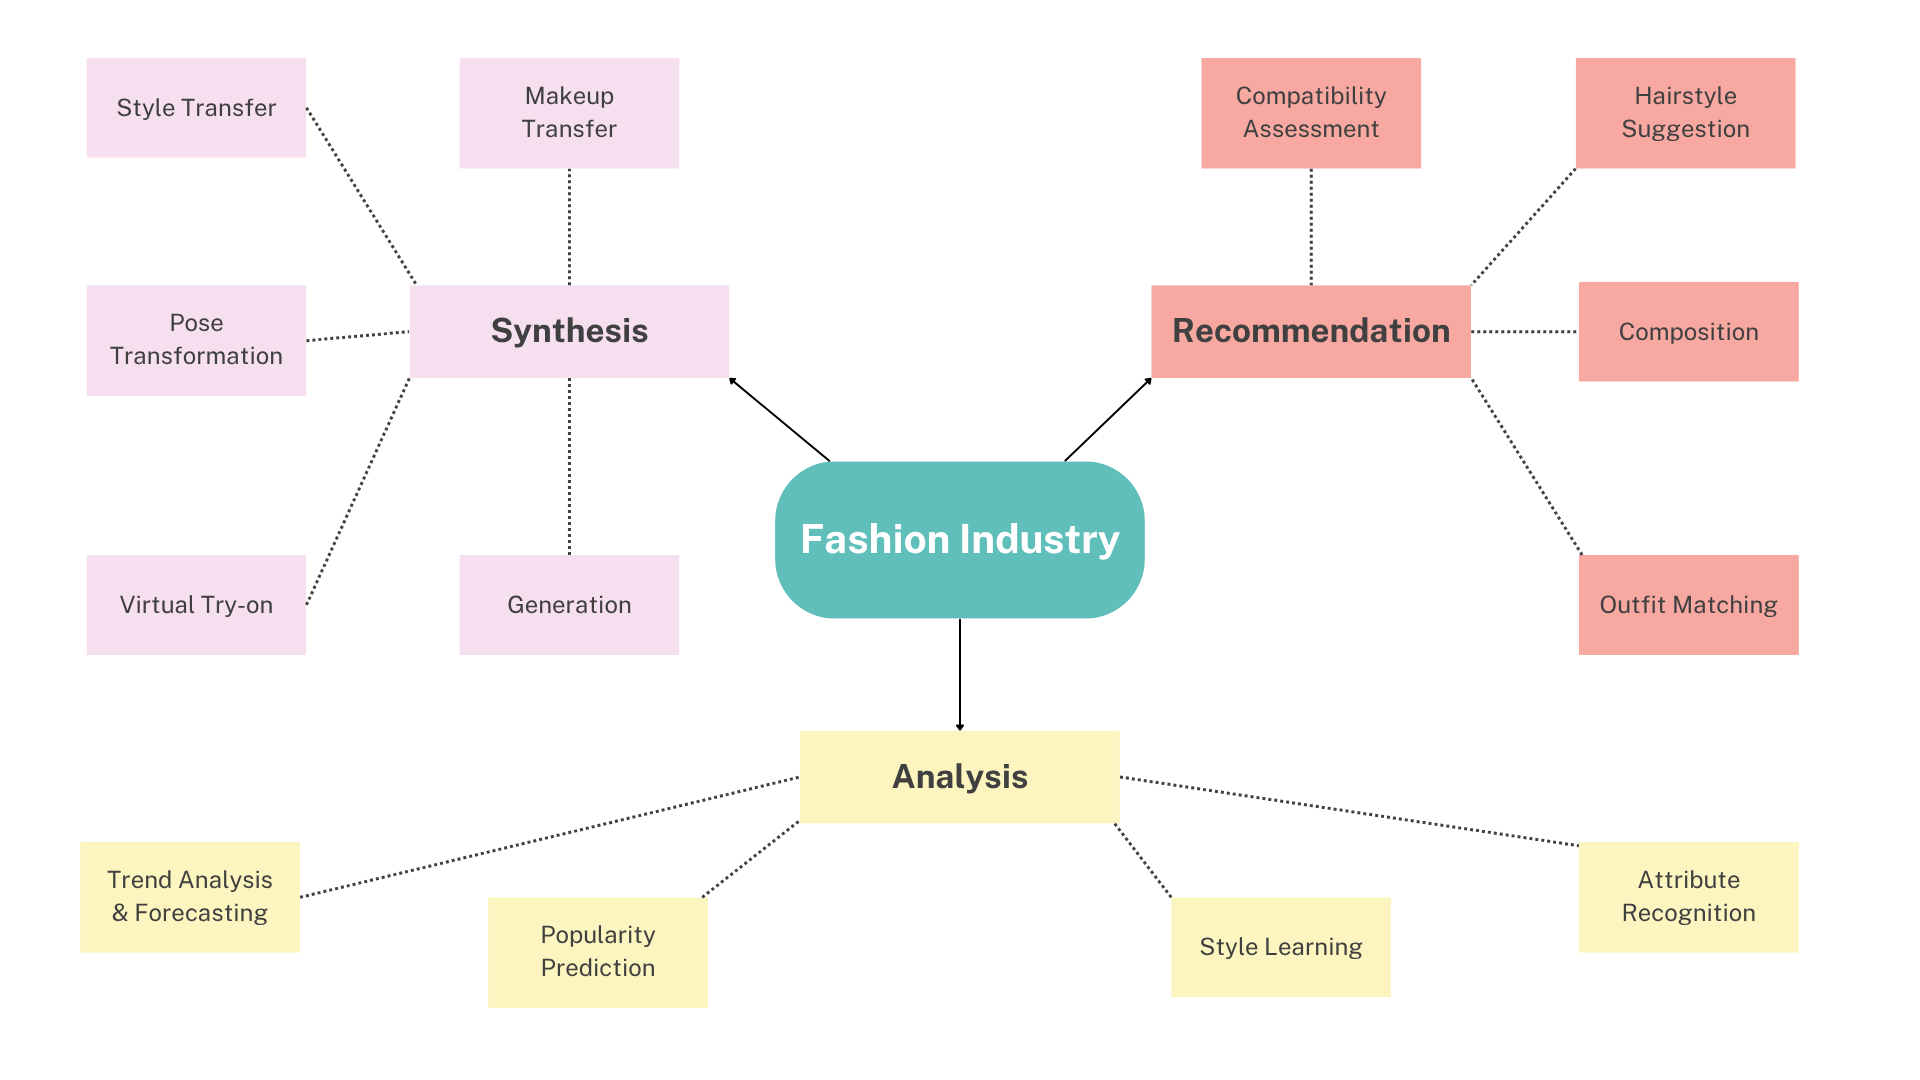
\includegraphics[width=\linewidth]{Abbildungen/fashion-areas.png}
  \caption{AI in Fashion (Mindmap)}
  \label{fig:fashion-areas}
\end{figure}

The goal of fashion recommendation is to automatically provide users with advice on what looks best on them and how to improve their style. This compatibility assessment is commonly associated with the task of outfit matching, where the overall collaboration between fashion items such as tops, bottoms, shoes, accessories is measured. \cite[cf.]{chen_survey_2023}

\section{Relevant Techniques in Outfit Matching and Compatibility Evaluation}

Outfit matching and compatibility evaluation combine principles from fashion theory, \acs{DL} and \acs{CV} to assess how well clothing items harmonize. This section explores key techniques, starting with foundational rules and progressing to computational models used in previous work.

\subsection{Techniques within Fashion Theory}

Compatibility evaluation among fashion items is typically modeled through fashion recommendation systems, which can broadly be divided into two categories: similar item recommendation and complementary recommendation. The former focuses on image retrieval techniques that suggest visually similar or identical fashion pieces. The latter aims to recommend items that complete or enhance a given outfit. \cite[cf.]{shirkhani_study_2023}

\vspace{0.5cm}

\textbf{Complementary Recommendation:}

\vspace{0.5cm}

This type of system includes three strategies. First, item recommendation predicts a single missing item based on a specific category. Second, outfit recommendation or outfit completion involves assembling a full outfit from scratch or adding items to an existing one. Third, capsule wardrobe generation seeks to propose a minimal yet versatile collection of items that can be mixed and matched into various outfits.

Complementary recommendation can further be distinguished based on context (e.g. product-based, scene-based, occasion-based) and evaluation scope (e.g. pair-wise, list-wise, set-wise).

\textbf{Context.}
Product-based methods assess the compatibility between items by analyzing their visual features, typically using product images. Scene-based approaches go a step further by incorporating contextual details such as the season, location or user-specific attributes. Finally, occasion-based recommendations tailor outfit suggestions to specific events, cultural settings or social contexts, ensuring relevance to the user's immediate needs.

\textbf{Evaluation.}
In terms of structure: pair-wise evaluation looks at two items at a time, list-wise methods consider a sequence of items and set-wise approaches treat the outfit as a whole, analyzing how well all the pieces work together.

\subsection{Techniques within \acs{ML}}

This section provides an overview of information that is foundational to this thesis. The methods are introduced both to establish a theoretical understanding and to contextualize their relevance within the review of related work and the implementation phase.

\vspace{0.5cm}

\textbf{\ac{CV}:}

\vspace{0.5cm}

In addressing the task of visually aware evaluation of the outfit composition, \acs{CV} is employed. \acs{CV} aims to create methods for computers to replicate the complexity of the human visual system by understanding digital images (e.g. photos, videos, other visual media) and extracting valuable information from them. \cite[cf.]{brownlee_deep_2019}

\vspace{0.5cm}

\textbf{\ac{DL}:}

\vspace{0.5cm}

In the context of this thesis, a \acs{DL} model, an algorithm that is modeled after the structure of the human brain, acts as a foundational element. These models consist of layers of interconnected neurons that process and transform input data. The weights of the connections between neurons in the network are adjusted over time to recognize patterns in data that are relevant to a specific task. Thereby, complex representations of data are automatically learned. \cite[cf.]{muller_introduction_2017}

\vspace{0.5cm}

\textbf{\ac{CNN}.}
Some popular \acs{DL} architectures include \acs{CNN}, which process images by applying small, learnable filters over pixel regions. These filters extract local features such as edges or textures. As the image passes through multiple convolutional layers, the network builds a hierarchical representation, with deeper layers capturing increasingly complex and abstract features useful for tasks like classification or detection.

\vspace{0.5cm}

\textbf{\ac{ResNet}.}
One of the key \acs{CNN} models in fashion is \acs{ResNet}. Its key feature is the use of \textcolor{red}{skip/residual connections} across one or more layers, which help mitigate the \textcolor{red}{vanishing gradient (incl. backpropagation)} problem in very deep networks. It uses building blocks and lets each block learn a modification (residual) to its input, rather than the desired underlying function. This allows gradients to flow backward. Therefore, this model can handle very deep networks (with over 100 layers: e.g. ResNet-50, ResNet-101, ResNet-152), making it suitable for feature extraction from complex fashion datasets where high accuracy is required. \cite[cf.]{he_deep_2015}

\vspace{0.5cm}

\textbf{\ac{DeCNN}.}
\acs{DeCNN} inverts the operations of \acs{CNN} to reconstruct high-dimensional data (e.g. image segmentation, object detection, image synthesis). It leverages deconvolutional layers and unpooling, recovers spatial details lost during downsampling and learns hierarchical representations critical for both low-level (e.g. deblurring) and high-level (e.g. segmentation) tasks. \cite[cf.]{zeiler_deconvolutional_2010}

\vspace{0.5cm}

\textbf{\ac{RelNNs}.}
\acs{RelNNs} addresses the task of relational reasoning. It is specifically designed to understand and compute pairwise relationships between objects or entities within data, showing how different parts of the input relate to each other. \cite[cf.]{sung_learning_2018}

\vspace{0.5cm}

\textbf{Siamese Network.}
A Siamese Network (Twin Network) is a neural network architecture designed for similarity learning. Its goal is to determine how alike or different two inputs of the same modality (e.g. images) are. This network consists of a pair of neural networks that share their weights and aim at computing similarity functions. It learns to compare pairs of inputs by mapping them into a feature space where similar samples are close and dissimilar samples are far apart. This approach is powerful in fashion scenarios where the task involves verifying whether two samples belong to the same class (e.g. similar style despite differences in type or color). \cite[cf.]{koch_siamese_2015}

\vspace{0.5cm}

\textbf{\ac{VSE}.}
These models map images and textual descriptions into a shared vector space. This enables cross-modal tasks such as image-text retrieval, caption generation and visual question answering. \acs{CLIP} is a specific implementation of a \acs{VSE}-like model including important advancements. Fashion\acs{CLIP} is domain-adapted version of \acs{CLIP} which is fine-tuned and tailored specifically for fashion-related tasks. \cite[cf.]{faghri_vse_2018}

\vspace{0.5cm}

\textbf{\ac{MLP}.}
One of the earliest models that is often being used to produce the final prediction, a compatibility score, is \acs{MLP}. \textcolor{red}{It is a multi-layer, fully connected, feedforward neural network capable of learning complex patterns through nonlinear transformations and iterative training.} \cite[cf.]{upgrad_overview_2023}

\vspace{0.5cm}

\textbf{Generative AI:}

\vspace{0.5cm}

Generative AI is another type of \ac{DL}. It creates new content (images, videos or text) based on patterns learned from existing data.

\vspace{0.5cm}

\textbf{\ac{Bi-LSTM}.}
A \acs{Bi-LSTM} network is an advanced type of \acs{RNN} and is designed for sequence modeling tasks. It processes sequential data in both forward and backward directions and combines their outputs to capture full context at every step. This architecture is especially powerful for tasks where understanding both past and future elements in a sequence is important. \cite[cf.]{huang_bidirectional_2015}

\vspace{0.5cm}

\textbf{\ac{GAN}.}
A \acs{GAN} is a framework where a generator and discriminator are trained in opposition. This results in a creation of highly realistic data. The process is unsupervised, game-theoretic and widely used for e.g. image synthesis, data augmentation, text-to-image generation, style transfer. \cite[cf.]{goodfellow_generative_2014}

\section{Previous Work and Related Research}

Current section provides an overview of 10 papers that were choosen out of a total of 54 in terms of their relevance to the use case. For all selected studies, their main goal and important technical elements were summarized. \vspace{0.5cm}

\textcolor{red}{explain the selection process?}
\textcolor{red}{remove hyperparameters later?}
\textcolor{red}{check if all methods / techniques are explained earlier}

\vspace{0.5cm}

\textbf{Pairwise Approach:}

\vspace{0.5cm}

Wang et al. present a system that can predict whether a set of clothing items representing an outfit looks good and explain why it does (not). The developed network uses a \acs{CNN} (\acs{ResNet} 50) and \acs{GAP} to extract features from images of clothing items at different levels of abstraction. These features range from basic details such as color and texture (early layers) to more complex ones such as style and category (later layers). The extracted features are then used to compare each outfit item with every other outfit item in a pairwise comparison matrix. \acs{MLP} then produces a score that reflects the final overall compatibility score. Thus, both visual and textual information is integrated using \acs{VSE} which allows the model to learn a common representation between them. Gradient values generated by backpropagation are used to identify problematic pairs and to provide an explanation of why an outfit fails, pinpointing specific issues. As loss functions, the model employs binary cross-entropy and contrastive loss. The training is supervised, uses labeled data and learns with negative sampling. The prediction of compatibility is evaluated using metrics such as \acs{AUC} and \acs{FITB} accuracy. The key hyperparameters mentioned include: initial \acs{LR}: 0.01, decay factor: 0.2 every 10 epochs, \acs{CNN} depth: 4 layers, \acs{MLP} depth: 2 layers. \cite[cf.]{wang_outfit_2019}

\vspace{0.5cm}

\textbf{Relational Approach:}

\vspace{0.5cm}

Moosaei et al. tackle the challenge of creating a system that could 1) work with any number of clothing items 2) without needing a specific order and 3) without relying on traditional labels. First, \acs{RelNNs} is used to treat each outfit as a "scene" and the items within it as "objects", thus learning how items relate to each other visually. After establishing the relationships, it combines them using \acs{MLP} to create a single score that indicates how well the outfit fits together. The authors also develop a more sophisticated version of the network that additionally incorporates textual information. DenseNet is used for visual feature extraction, one-hot encoding for textual features. The model uses cross-entropy loss. The training is supervised. The evaluation uses \acs{AUC} and \acs{FITB} accuracy. The key hyperparameters mentioned include: \acs{LR}: 0.001, batch size: 64, dropout rate: 0.35, epochs: 19, optimizer: Adam, \acs{MLP} depth: 4 layers (number of filters: 512, 512, 256, 256) + 3 layers (number of filters: 128, 128, 32). \cite[cf.]{moosaei_fashion_2020}

\vspace{0.5cm}

\textbf{Generative Approach and Template Generation:}

\vspace{0.5cm}

Liu et al. aim not only to measure compatibility but also to generate a "compatible template" that could help in understanding why certain pairings succeed or fail. The authors trained a \acs{GAN} on a massive dataset of clothing images paired with detailed textual descriptions to create a richer understanding of clothing compatibility. The architecture integrates down-sampling, multi-modal fusion and up-sampling. Convolutional layers are used for visual encoding, TextCNN for textual. The network learns to generate preliminary visual representations (templates) of what a compatible clothing item should look like based on a given one. \acs{AUC} and \acs{MRR} are used as metrics for evaluating the model. The \acs{LR} was set to 0.0002. \cite[cf.]{liu_mgcm_2020}

\vspace{0.5cm}

\textbf{Generative Approach:}

\vspace{0.5cm}

In another research, Moosaei et al. show a model used to generate compatible fashion items for an (incomplete) outfit. The developed model consists of two parts. The \acs{GAN} takes as input a partial outfit (images) along with a specified missing clothing item category (textual) and creates several potential outfit combinations. A compatibility network (\acs{CNN} + \acsp{MLPs} + \acs{RelNNs}) checks if the generated item fits well with the rest of the outfit by identifying patterns in the relationships between items. It learns what makes different clothing items match each other based on their contextual relevance (relationships) and their visual aesthetics by incorporating the initial outfit input into its training. As a loss function, the model employs cross-entropy loss among others. Training is supervised for compatibility network and min-max game for \acs{GAN}. The prediction is evaluated using inception score, multi-scale structural similarity and compatibility score. \cite[cf.]{moosaei_outfitgan_2022}

\vspace{0.5cm}

\textbf{Graph-based Approach and Try-on Approach:}

\vspace{0.5cm}

Zheng et al. address item-by-item matching (collocation) and overall outfit appearance (try-on). Both of these perspectives are combined in a network to give a better evaluation of outfit compatibility. The developed model consists of two parts. \cite[cf.]{zheng_collocation_2021}

\begin{enumerate}
  \item The first part looks at each clothing item individually and checks how well they match with each other. This approach uses a disentangled \acs{GCN} and includes nodes (each representing clothing items), edges (showing the connections between items), condition masks (acting like filters that separate out different features of clothing items) and an attention mechanism (deciding which features are more crucial for determining if items match). Convolutional layers are used for visual features, \acs{ResNet}-like architecture for try-on images. 
  \item The second part imagines how the whole outfit would look when worn together and outputs the final try-on compatibility score. Thereby, the authors apply knowledge distillation and train a "teacher" network using available try-on images before transferring knowledge to a "student" network. This second network predicts how the outfit would look without the need for actual try-on images. Furthermore, item category information (such as top, bottom, etc.) is incorporated to understand the context of the outfit.
\end{enumerate}

In this paper, cross-entropy is chosen as a loss function, while the Kullback-Leibler divergence and L1 regularization are used as regularization terms. Instance normalization is applied. The training is semi-supervised with mutual learning strategy. The prediction of compatibility is evaluated using metrics such as \acs{AUC}, \acs{MRR}, \acs{HR} @1, @10, @100, @200. The key hyperparameters mentioned include: \acs{LR}: 0.0002, batch size: 32, optimizer: Adam, activation function: \acs{ReLU} (and Tanh), \acs{GCN} depth: one 1-strided convolutional layer and four 2-strided convolutional layers (number of filters: 32, 64, 128, 256, and 512, respectively), teacher network depth: same as \acs{GCN} for encoder + transform block composed of 6 residual blocks + decoder with four 2-strided deconvolutional layers and one 1-strided convolutional layer (number of filters: 32, 64, 128, 256, 512, 512, 512, 512, 512, 512, 512, 256, 128, 64, 32 and 3, respectively). \cite[cf.]{zheng_collocation_2021}

\vspace{0.5cm}

\textbf{Graph-based Approach:}

\vspace{0.5cm}

Work done by Guan et al. presents a system designed to automate the assessment of outfit compatibility while dealing with irregular attribute labels, information loss during disentanglement and combining different levels of information. The system tackles this through a three-stage methodology: \cite[cf.]{guan_partially_2022}

\begin{enumerate}
  \item It leverages a pre-trained model (\acsp{ResNet} 18) to extract visual features from each clothing item. \acsp{MLPs} are applied to break these features down into attributes (partially supervised disentangled learning). Despite the fact that the generated attribute labels are irregular, this partially supervised approach is used to guide the attribute-level learning.
  \item To prevent losing information during breakdown, the authors introduce two strategies: orthogonal residual embedding layers (layers that reintroduce missing information) and visual representation reconstruction (a \acs{DeCNN} that reconstructs the original image from fragmented attributes).
  \item The system builds a graph where nodes represent fashion items and edges represent compatibility relationships (e.g. "matches", "does not match", "requires modification"). Hierarchical \acs{GCN} is implemented to model the relationships between clothing items, considering both attribute-level and item-level compatibility. The final compatibility score is derived from the combination of both results.
\end{enumerate}

In this paper, cross-entropy is chosen as a loss function, while orthogonal regularization is used as a regularization term. The evaluation uses \acs{AUC} and \acs{FITB} accuracy. The key hyperparameters mentioned include: \acs{LR}: 0.0001, batch size: 32, optimizer: Adam, \acs{GCN} depth: 1 layer, \acs{DeCNN} depth: 5 transposed layers (output dimension: 256), \acsp{MLPs} depth: 2 layers (for each label with output dimension: 64), activation functions: LeakyReLU, \acs{ReLU}, Tanh. \cite[cf.]{guan_partially_2022}

\vspace{0.5cm}

\textbf{Colors and Textures:}

\vspace{0.5cm}

Kim et al. implement a model that can learn from unlabeled data using \acs{SCL} and suggest items that complement each other based on shared color palettes and textures. On the one hand, the model learns to predict the distribution of colors present in images and to recognize color patterns. On the other hand, it learns to identify and recognize different textures (such as stripes, polka dots, etc.). Additionally, in order to filter out irrelevant information (e.g. shape), the model focuses on smaller, independent image patches and learns to identify the types of colors and textures present within these patches. The architecture consists of \acs{CNN} (\acs{ResNet} 50) and separate projection heads for sub-tasks. Contrastive loss (for shapeless local patch discrimination, texture discrimination) is chosen as a loss function, while the Kullback-Leibler divergence (for RGB histograms) and L1 regularization are used as regularization terms. The prediction is evaluated using \acs{AUC}, \acs{FITB} accuracy, recall@K. The key hyperparameters mentioned include: \acs{LR}: 0.00005, optimizer: Adam, activation function: \acs{ReLU}, epochs: 150, heads depth: two fully connected layers. \cite[cf.]{kim_self-supervised_2020}

\vspace{0.5cm}

\textbf{Styles and Textures:}

\vspace{0.5cm}

Dong et al. present a system that can automatically generate matching clothing items while considering style and texture using \acs{SSL}. This is done without requiring pairs of outfits that already match, instead mapping an input image of a clothing item to a complementary image. The network utilizes three main parts: \cite[cf.]{dong_towards_2025}

\begin{enumerate}
  \item First component (discriminator with \acs{ResNet} backbon and \acsp{MLPs}) helps the system understand the style and texture representations of the input clothing. Later on it ensures that the synthesized clothing is compatible with the input clothing in terms of style and texture.
  \item The second component (dual discriminator) ensures that the generated images are realistic and visually coherent. One discriminator is designed to favor real images (positive samples) and assigns high scores to latent codes produced by the encoding network, while the other discriminator favors generated images (negative samples) and assigns high scores to latent codes produced by the mapping network. Conversely, the first discriminator assigns low scores to latent codes from the mapping network, and the second assigns low scores to latent codes from the encoding network.
  \item Build upon \acs{GAN} inversion, the last component (generator) uses a pre-trained model (StyleGAN) to understand the basic structure of clothing. It then applies style and texture information to generate a matching image, guided by the DST and dual discriminator losses.
\end{enumerate}

\vspace{0.5cm}

\textbf{Body Shape:}

\vspace{0.5cm}

Pang et al. designed a model that generates outfit recommendations that prioritize both visual compatibility and body shape suitability. This is achieved through a layered architecture that incorporates: \cite[cf.]{pang_learning_2024}

\begin{enumerate}
  \item Seven body shape representations with 3D body models, measurements and front-view images captured from multiple angles for each body shape. These are used to train the model to understand the overall silhouette using \acs{SMPL} and \acs{ResNet}.
  \item This part extracts visual features from images that show how an outfit looks when worn (available or generated with M-VTON) using \acs{ResNet}. It also generates textual descriptions of clothing attributes using \acs{GloVe}. Both are then represented as vector representations.
  \item The final part of the model combines body shape representation and outfit representation into a single, unified representation. Cross-modal attention is used to identify correlations between body shape and outfit attributes, focus on the most relevant features when making recommendations and provide explanations for why an outfit is recommended.
\end{enumerate}

Thereby, binary cross-entropy loss is chosen as a loss function. The evaluating metrics include \acs{AUC}, mean average precision, average per-class precision, recall, F1 score, average overall precision. The key hyperparameters mentioned are: \acs{LR}: 0.1, batch size: 10, optimizer: SDG, activation function: \acs{ReLU}, weight decay: 0.0005, momentum: 0.9. \cite[cf.]{pang_learning_2024}

\vspace{0.5cm}

\textbf{Occasion:}

\vspace{0.5cm}

In their work, Vo et al. create a system that can tell if different clothing items are compatible for specific occasions beyond simple style matching. The authors designed a framework with three main parts: \cite[cf.]{vo_efficient_2023}

\begin{enumerate}
  \item \acs{Bi-LSTM} analyzes the entire outfit as a sequence (like words in a sentence) and learns how different clothing items relate to each other.
  \item \acs{ResNet} 50 extracts visual features from clothing images and \acs{VSE} connects them to textual descriptions (one-hot encoded) to understand visual style and matching.
  \item The last part focuses specifically on recognizing if an outfit is suitable for a particular occasion. It uses an auxiliary classifier with global average pooling, fully connected layers and softmax to classify outfits based on occasions.
\end{enumerate}

The system is evaluated using metrics such as \acs{AUC} and \acs{FITB} accuracy. As a loss function, it employs triplet loss and cross-entropy loss among others. The key hyperparameters mentioned include: batch size: 10, initial \acs{LR}: 0.2, then changed by a factor of 2 for every two epochs. \cite[cf.]{vo_efficient_2023}
